% =========================================================================
% AI-Assisted Aircraft Conceptualization:
% Preliminary Design of a Tail-Sitter UAV
%
% Build:  latexmk -pdf main.tex     (or: pdflatex + bibtex + pdflatex x2)
% =========================================================================
\documentclass[11pt,a4paper]{article}

\usepackage[T1]{fontenc}
\usepackage[utf8]{inputenc}
\usepackage{lmodern}
\usepackage[margin=2.5cm]{geometry}
\usepackage{amsmath,amssymb}
\usepackage{graphicx}
\usepackage{booktabs}
\usepackage{multirow}
\usepackage{tabularx}
\usepackage{caption}
\usepackage{subcaption}
\usepackage[round,authoryear]{natbib}
\usepackage{tikz}
\usetikzlibrary{arrows.meta,positioning,shapes.geometric}
\usepackage{xcolor}
\usepackage{enumitem}
\usepackage[hidelinks]{hyperref}

% --- editorial helpers (remove before submission) ------------------------
\newcommand{\todopaper}[1]{\textcolor{red}{[TODO: #1]}}
\newcommand{\citeneeded}{\textcolor{red}{[citation needed]}}

% --- shorthand ------------------------------------------------------------
\newcommand{\code}[1]{\texttt{#1}}
\graphicspath{{figures/}}

\title{\textbf{AI-Assisted Aircraft Conceptualization:\\
Preliminary Design of a Tail-Sitter UAV}}

\author{%
  Onur Tuncer$^{1,}$\thanks{Corresponding author: \texttt{onur.tuncer@itu.edu.tr}}
  \and Ahmet G\"une\c{s}$^{2}$
  \and \c{C}a\u{g}lar U\c{c}ler$^{3}$\\[1ex]
  \small $^{1}$Istanbul Technical University, Faculty of Aeronautics and Astronautics, Istanbul, T\"urkiye\\
  \small $^{2}$\todopaper{affiliation of Ahmet G\"une\c{s}}\\
  \small $^{3}$\todopaper{affiliation of \c{C}a\u{g}lar U\c{c}ler}%
}
\date{}

\begin{document}
\maketitle

\begin{abstract}
The conceptual design phase fixes most of an aircraft program's key
decisions while information is scarcest, and it remains dominated by
slow, experience-driven, iterative workflows. Existing applications of
artificial intelligence (AI) to aircraft design are fragmented ---
surrogate aerodynamics, isolated optimizers, code assistance --- and no
structured methodology yet integrates AI across the complete conceptual
design process while preserving physics-based rigor. This paper
proposes such a methodology, in which a large-language-model (LLM)
agent acts as an engineering collaborator inside a version-controlled
design repository: every physical model is deterministic, configured,
and under regression test; the AI writes, refactors, and re-converges
those models under natural-language direction from human engineers, and
every design decision is captured as an architecture decision record
with full git-level provenance of AI contribution. Guardrails --- a
machine-readable project constitution, a one-way dataflow pipeline with
typed hand-offs, pinned design-point regression tests, and continuous
integration that re-executes the entire design on every change ---
ensure that the AI accelerates iteration without ever becoming the
source of an engineering number. The methodology is demonstrated on the
conceptual design of a small electric tail-sitter VTOL UAV (single
ducted fan, jet vanes): starting from mission requirements, the
human--AI team produced a converged, COTS-frozen 2.52\,kg design point
--- thirteen tagged design snapshots, eighteen recorded architecture
decisions, and a sixteen-stage analysis pipeline spanning sizing,
aerodynamics, control authority, vibration, thermal, CAD, and CFD
hand-off --- in under three weeks of part-time work, while independent
expert review remained an integral, documented part of the loop. The
resulting workflow is aircraft-agnostic and directly transferable to
other rapidly iterating aerospace development programs.
\end{abstract}

\noindent\textbf{Keywords:} artificial intelligence; aircraft
conceptual design; tail-sitter UAV; large language models; agentic
workflows; multidisciplinary design

\section{Introduction}
\label{sec:intro}

\subsection{Research need and gap}

The conceptual design phase establishes the foundation of every
aircraft development program by defining the overall configuration,
mission feasibility, propulsion architecture, structural layout,
subsystem selection, and overall system performance. These early-stage
decisions rely heavily on preliminary sizing calculations, engineering
heuristics, multidisciplinary trade-off analyses, and numerous design
iterations, despite limited available information
\citep{corrado2022,karali2024surrogate}. In recent years, artificial
intelligence (AI) has demonstrated considerable potential in supporting
individual engineering tasks; however, existing applications remain
fragmented and are typically limited to isolated activities such as
surrogate modeling, geometry generation, programming assistance,
optimization, or document preparation
\citep{karali2024mdo,du2026,pliakos2025}. There is still no structured
methodology that systematically integrates AI into the complete
conceptual aircraft design process while preserving physics-based
engineering calculations, multidisciplinary reasoning, and engineering
verification. This need is particularly critical for UAV development,
where rapidly evolving operational requirements, frequent design
updates, and short development cycles demand conceptual design
iterations significantly faster than those traditionally adopted in
conventional aircraft programs \citep{karali2023,shakeri2018}.

A qualitatively new opportunity has emerged with large language model
(LLM) based \emph{agentic} coding tools, which can read, write,
execute, and test an entire engineering codebase under natural-language
direction. Unlike the surrogate-model and optimizer literature, which
replaces expensive physics with learned approximations, an LLM agent
can operate one level higher: it can \emph{build and maintain} the
deterministic physics toolchain itself, propose and implement design
changes across every affected discipline simultaneously, and document
the reasoning --- while the engineering numbers continue to come
exclusively from transparent, testable, physics-based code. How to
harness this capability without sacrificing rigor, traceability, and
verification is, to the authors' knowledge, unaddressed in the aircraft
design literature.

\subsection{Proposed methodology}

This study presents an AI-assisted conceptual aircraft design
methodology that supports the complete early-stage development process
from mission definition to a validated conceptual configuration. The
methodology integrates preliminary aircraft sizing, propulsion sizing,
energy storage estimation, subsystem and equipment selection,
configuration development, structural considerations, and
multidisciplinary engineering evaluations within a unified iterative
framework. Artificial intelligence functions as an engineering
collaborator that accelerates engineering reasoning, alternative
generation, knowledge synthesis, component evaluation, technical
documentation, and design-space exploration, while analytical
calculations remain the basis of all engineering decisions. Numerical
analyses, computational simulations, and external expert findings are
continuously incorporated into successive design iterations, enabling
the conceptual design to evolve through evidence-based refinement
rather than linear development.

The methodology is realized concretely as a \emph{governed
human--AI--repository loop}: the design lives entirely in a
version-controlled repository whose architecture (configuration
$\rightarrow$ physics library $\rightarrow$ notebook pipeline
$\rightarrow$ typed hand-offs $\rightarrow$ CAD/CFD consumers) is
itself part of the method; the AI agent works inside that repository
under a machine-readable set of engineering rules; and every change is
gated by human review, architecture decision records, pinned
design-point regression tests, and continuous integration that
re-executes the full design. To demonstrate applicability, a
tail-sitter VTOL UAV is developed as an illustrative case study,
covering the process from mission requirements to preliminary sizing,
subsystem selection, configuration development, commercial
component freeze, and hand-off to higher-fidelity validation.

The work is guided by the following research question:

\begin{quote}
\textbf{RQ:} \emph{How can AI accelerate conceptual aircraft design
while preserving physics-based engineering rigor?}
\end{quote}

\subsection{Main contributions}

The primary contribution of this work is the introduction of a
structured AI-assisted methodology for conceptual aircraft design that
integrates preliminary engineering calculations, multidisciplinary
subsystem selection, engineering knowledge management, numerical
analyses, and iterative design refinement into a single coherent
workflow. Unlike existing AI applications that support isolated
engineering tasks, the proposed methodology formalizes the interaction
between human engineering expertise, an LLM-based AI agent, analytical
models, and validation activities throughout the conceptual design
process --- including the guardrails (design-point regression pins,
one-way dataflow, decision records, standing-finding discipline) that
make AI acceleration compatible with engineering accountability. The
framework is aircraft-independent and can be adapted to a wide range of
aerospace platforms that require rapid, multidisciplinary conceptual
development.

As a second contribution, the paper demonstrates the practical
implementation of the methodology through the conceptual design of a
tail-sitter VTOL UAV, resulting in a complete preliminary sizing
procedure, propulsion system selection, onboard equipment architecture,
and configuration development, together with quantitative process
evidence extracted from the project's own git history: the share of
AI-co-authored engineering commits, the cadence of design-point
snapshots, and the mechanisms by which errors were caught. Furthermore,
the tail-sitter case study provides application-specific engineering
insights into the conceptual development of this unconventional
aircraft configuration, illustrating how AI-assisted multidisciplinary
workflows can reduce development effort while maintaining engineering
rigor, traceability, and design quality.

The remainder of the paper is organized as follows.
Section~\ref{sec:related} reviews AI applications in conceptual
aircraft and UAV design and motivates the tail-sitter as a validation
case. Section~\ref{sec:method} presents the methodology.
Section~\ref{sec:results} reports the case study results and process
metrics and discusses them against the research question.
Section~\ref{sec:conclusions} concludes.

\section{AI and Conceptual Design}
\label{sec:related}

This review covers three linked needs: why AI-assisted conceptual
design is needed in aircraft and especially UAV development, which AI
tools and frameworks already exist, and why a tail-sitter VTOL UAV is a
useful validation case relative to other eVTOL architectures.

\subsection{Design need}

Aircraft conceptual design is still constrained by long, costly,
iterative workflows that must reconcile aerodynamics, structures,
propulsion, stability, manufacturing, and mission requirements early,
when most key decisions are fixed
\citep{karali2024surrogate,corrado2022,lukyanov2024}. Conventional
sequential methods depend heavily on designer experience and
low-fidelity semi-empirical models, which are especially weak for UAVs
because many UAV sizes, Reynolds-number regimes, and unconventional
layouts fall outside the historical data behind those regressions
\citep{karali2024surrogate,lukyanov2024}.

UAV design sharpens this need because UAVs can adopt tailless,
blended-wing, morphing, tandem, canard, and other nontraditional
configurations that demand broader design-space exploration and tighter
coupling between mission definition and vehicle architecture
\citep{karali2024surrogate,ivanova2025,lukyanov2024}. High-fidelity CFD
and finite-element analyses improve realism, but thousands of
evaluations across optimization loops make direct early-stage use
computationally prohibitive, motivating automation, surrogates, and
concurrent multidisciplinary design optimization (MDO) workflows
\citep{karali2024surrogate,wang2023,pliakos2025,leng2024}.

\begin{itemize}[nosep]
\item Early MDO detail is needed to reduce late development setbacks
  and resolve the conceptual-stage ``design paradox'' while design
  freedom remains high \citep{corrado2022}.
\item UAV programs need faster iteration because competition, budget
  limits, and expanding mission complexity make broad manual concept
  trades increasingly impractical
  \citep{karali2023,pliakos2025,shakeri2018}.
\item AI is increasingly relevant because modern UAVs already rely on
  autonomy, real-time decision-making, and mission adaptation under
  battery and payload constraints
  \citep{ivanova2025,sai2023,mcenroe2022}.
\end{itemize}

\subsection{AI tools and frameworks}

The literature points to a clear pattern: AI in conceptual aircraft
design is used less as a replacement for physics than as a
computational amplifier around physics-based models, MDO loops, and
design iteration. The dominant tools are surrogate models for
aerodynamics, structural mass, and sometimes radar cross-section;
evolutionary or multiobjective optimizers; automated geometry/CFD
pipelines; and data-mining or multi-fidelity schemes that reduce
coupling and computational burden
\citep{karali2024surrogate,leng2024,pliakos2025}.

Reported frameworks already support configuration selection, early
sizing, and iterative refinement. AI-supported UAV conceptual design
frameworks compare alternative configurations using learned
disciplinary models, feed optimized results back into sizing, and can
cut runtime dramatically; one deep-learning surrogate framework
reported more than three orders of magnitude computational-time
improvement over traditional methods \citep{karali2024surrogate}. The
methodological frontier is widening toward uncertainty-aware MDO,
digital twins, generative AI, and automated data-generation pipelines
that make high-quality training data easier to produce
\citep{karali2024surrogate,wang2023,du2026,pliakos2025}.

Table~\ref{tab:methodclasses} summarizes representative AI-supported
methodology classes reported for aircraft and UAV conceptual design.

\begin{table}[htbp]
\centering
\caption{Representative AI-supported methodology classes reported for
aircraft and UAV conceptual design.}
\label{tab:methodclasses}
\small
\begin{tabularx}{\textwidth}{@{}lXX@{}}
\toprule
\textbf{Method class} & \textbf{What it supports} &
\textbf{Representative evidence} \\
\midrule
ANN / deep surrogates &
Fast aerodynamics, mass, RCS prediction for concept comparison and
sizing &
AI-driven UAV frameworks use learned aerodynamics, structural mass,
and RCS models in early design \citep{karali2024surrogate} \\
\addlinespace
Evolutionary / GA / DE / multiobjective optimization &
Configuration search, wing optimization, takeoff-weight reduction,
trade-space exploration &
GA{+}ANN wing optimization and DE-based UAV optimization are
established \citep{boutemedjet2019,komarov2024} \\
\addlinespace
Multi-fidelity / data mining &
Variable screening, disciplinary decoupling, cheap-to-expensive
optimization progression &
Multi-fidelity data mining uses low-cost data first, then CFD
fine-tuning \citep{leng2024} \\
\addlinespace
Automated CFD pipelines &
Rapid geometry, meshing, solver setup, dataset generation &
Python-based preprocessing reduces turnaround to minutes with
sub-5\% deviation from expert setups \citep{pliakos2025} \\
\addlinespace
Generative / emerging AI &
Parameterization, predictive modeling, training facilitation,
constraint handling &
GenAI applications now span VAE, GAN, diffusion, and transformer
approaches \citep{du2026} \\
\addlinespace
LLM / agentic coding assistants &
Building and maintaining the analysis toolchain itself;
multidisciplinary change propagation; documentation &
This work; general-purpose agentic tools \citep{anthropic2025claudecode} \\
\bottomrule
\end{tabularx}
\end{table}

\begin{itemize}[nosep]
\item Reinforcement learning is widely used in AI-integrated UAV
  systems, while federated and distributed learning frameworks are
  emerging quickly \citep{sai2023}.
\item AI toolchains increasingly include libraries, frameworks, and
  edge/embedded deployment pathways, not just offline design
  optimizers \citep{sai2023,mcenroe2022}.
\item Current gaps remain important: many studies still focus on
  airfoils or wings rather than full-aircraft models, and robust
  treatment of uncertainty, unconventional configurations, and broader
  objective sets is still developing
  \citep{karali2024surrogate,wang2023,lukyanov2024}.
\end{itemize}

Notably, none of the surveyed frameworks employs AI at the
\emph{workflow} level --- as an agent that authors, verifies, and
evolves the design toolchain and its documentation under human
direction. That is the niche addressed by the present methodology.

\subsection{Tail-sitters versus eVTOLs}

Tail-sitter VTOL UAVs are a strong validation case because they force a
conceptual design method to address the hardest coupling in VTOL
design: hover, wing-borne cruise, and the transition between them.
Recent VTOL design studies argue that transition and climb are often
oversimplified in conceptual design even though they strongly drive
motor and battery sizing \citep{kaneko2024}. For tail-sitters
specifically, nonlinear dynamics during transition are a central
limitation, with widely varying speed and attitude, unstable
long-period behavior in some regimes, and controller sensitivity to
uncertainty \citep{yang2024}.

Against that difficulty, tail-sitters offer a simpler airframe than
many other eVTOL classes. Compared with tilt-rotor or dual-system
eVTOLs, tail-sitter eVTOLs remove tilting mechanisms and redundant
propulsors, which can reduce structural and mechanical complexity
\citep{yang2024}. But that simplicity trades for harder transition
physics: the aircraft must sustain pitch authority through a full
$90^{\circ}$ rotation, propulsors must provide both high vertical
thrust and efficient forward-flight operation, and oblique inflow
during transition can excite propeller vibration \citep{yang2024}.

\begin{itemize}[nosep]
\item Trajectory-coupled optimization materially matters for
  tail-sitters: simultaneous design-and-trajectory optimization reduced
  energy by 29\% versus uncoupled optimization in one tail-sitter
  delivery case \citep{kaneko2024}.
\item Optimized transition control improves operations, with reduced
  transition time and altitude excursion relative to traditional
  linear transition methods \citep{yang2024}.
\item A tail-sitter validation example is methodologically valuable
  because it stress-tests whether an AI-assisted conceptual design
  framework can integrate physics, controls, propulsion, and sizing in
  one loop rather than treating configuration choice and transition
  performance separately \citep{kaneko2024}.
\end{itemize}

Taken together, the literature supports an AI-assisted conceptual
design methodology that augments physics-based analysis rather than
replacing it, is especially justified for UAVs with unconventional
configurations, and is well validated by a tail-sitter VTOL case
because tail-sitters expose exactly the multidisciplinary and
transition-coupled trade-offs that simpler conceptual methods tend to
miss.

\section{Method}
\label{sec:method}

The methodology's central idea is a strict division of labor between
three actors, mediated by a version-controlled repository that is the
single source of truth for the design
(Fig.~\ref{fig:workflow}):

\begin{enumerate}[nosep,label=(\roman*)]
\item \textbf{Deterministic physics code} is the \emph{only} source of
  engineering numbers. Every sizing relation, mass model, and margin
  check is transparent, configured Python under regression test. No
  quantity used in a design decision is ever generated by the language
  model itself.
\item \textbf{The AI agent} --- an LLM-based agentic coding tool
  \citep{anthropic2025claudecode} with full read, write, and execute
  access to the repository --- writes, refactors, and re-converges
  that code,
  propagates design changes across every affected discipline, drafts
  decision records and documentation, and executes the analysis
  pipeline. It is an engineering \emph{collaborator}, not an oracle:
  its contributions are ordinary commits subject to the same review
  and testing gates as human-written ones.
\item \textbf{Human engineers} set requirements, issue design
  directives in natural language, review every change (via pull
  requests), perform independent expert review of the evolving design,
  and accept or reject each recorded decision.
\end{enumerate}

Sections~\ref{sec:pipeline}--\ref{sec:iteration} describe the four
pillars that make this collaboration rigorous: a one-way analysis
pipeline, a machine-readable governance layer, a verification harness
that the AI cannot silently bypass, and an interaction protocol with
full provenance.

\begin{figure}[htbp]
\centering
\resizebox{\textwidth}{!}{%
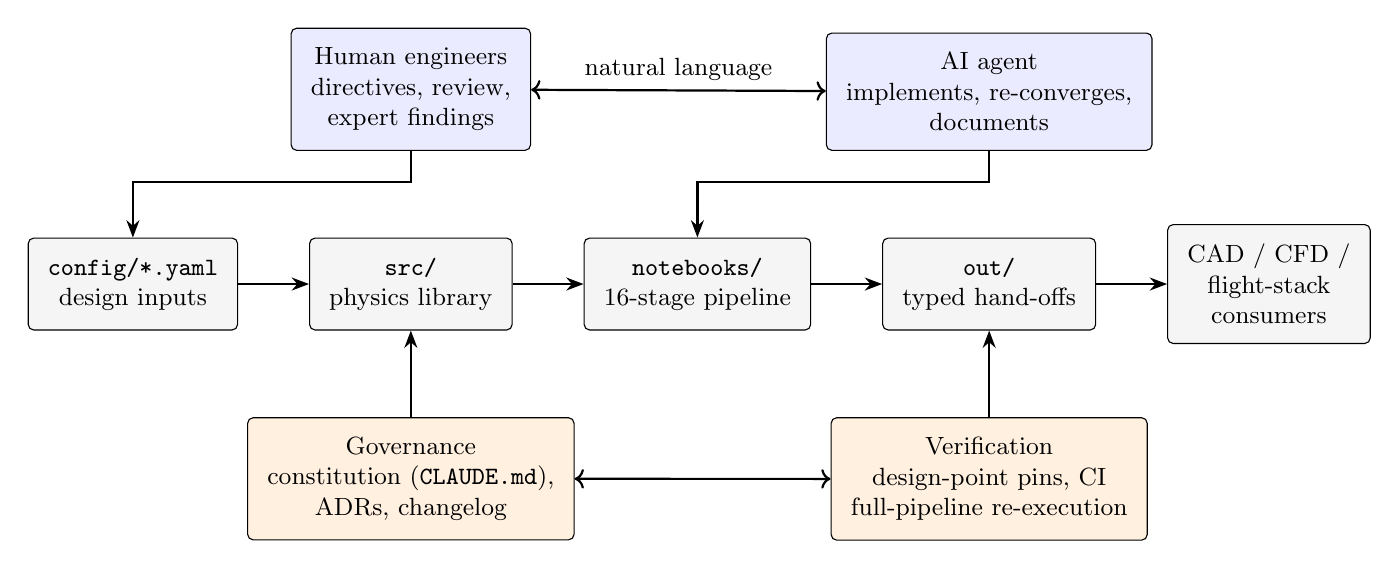
\begin{tikzpicture}[
  font=\small,
  node distance=5mm and 9mm,
  box/.style={draw, rounded corners=2pt, align=center, minimum height=8mm,
              inner sep=2.5mm, fill=gray!8},
  actor/.style={draw, align=center, minimum height=8mm, inner sep=2.5mm,
                fill=blue!8, rounded corners=2pt},
  gate/.style={draw, align=center, minimum height=8mm, inner sep=2.5mm,
               fill=orange!12, rounded corners=2pt},
  arr/.style={-{Stealth[length=2.2mm]}, thick}
]
% pipeline row
\node[box] (config) {\code{config/*.yaml}\\design inputs};
\node[box, right=of config] (src) {\code{src/}\\physics library};
\node[box, right=of src] (nb) {\code{notebooks/}\\16-stage pipeline};
\node[box, right=of nb] (out) {\code{out/}\\typed hand-offs};
\node[box, right=of out] (cfd) {CAD / CFD /\\flight-stack\\consumers};
\draw[arr] (config) -- (src);
\draw[arr] (src) -- (nb);
\draw[arr] (nb) -- (out);
\draw[arr] (out) -- (cfd);
% actors row
\node[actor, above=11mm of src] (human) {Human engineers\\directives, review,\\expert findings};
\node[actor, above=11mm of out] (ai) {AI agent\\implements, re-converges,\\documents};
\draw[arr, <->] (human) -- node[above]{natural language} (ai);
\draw[arr] (ai.south) -- ++(0,-4mm) -| (nb.north);
\draw[arr] (human.south) -- ++(0,-4mm) -| (config.north);
% gates row
\node[gate, below=11mm of src] (gov) {Governance\\constitution (\code{CLAUDE.md}),\\ADRs, changelog};
\node[gate, below=11mm of out] (ver) {Verification\\design-point pins, CI\\full-pipeline re-execution};
\draw[arr, <->] (gov) -- (ver);
\draw[arr] (gov.north) -- ++(0,4mm) -| (src.south);
\draw[arr] (ver.north) -- ++(0,4mm) -| (out.south);
\end{tikzpicture}%
}
\caption{The governed human--AI--repository loop. Engineering numbers
flow only left-to-right through the deterministic pipeline (top row);
the AI agent and human engineers modify the repository under the
governance and verification gates (bottom row).}
\label{fig:workflow}
\end{figure}

\subsection{The design repository as a one-way analysis pipeline}
\label{sec:pipeline}

All design knowledge lives in one repository with a strictly one-way
dataflow:
\begin{equation*}
\code{config/} \;\rightarrow\; \code{src/} \;\rightarrow\;
\code{notebooks/} \;\rightarrow\; \code{out/} \;\rightarrow\;
\text{CAD/CFD/flight-stack consumers.}
\end{equation*}
Every physical parameter --- mission times, aerodynamic limits,
battery properties, structural factors --- lives in commented YAML
configuration files with a written rationale; the Python physics
library contains \emph{no} magic numbers. Jupyter notebooks are thin
orchestration only (parameters, module calls, interpretation); all
physics, plotting, and reporting code lives in the importable library,
so the entire design is reproducible headlessly and testable by unit
tests. Each pipeline stage writes typed YAML/JSON hand-off files that
downstream stages read, and no stage ever writes back upstream. In the
case study this pipeline comprises sixteen notebook stages
(Table~\ref{tab:pipeline}), executed in dependency order.

This architecture is not incidental to the AI methodology --- it is
what makes an LLM agent safe to employ. Because the dataflow is
one-way and fully regenerable from \code{config/}, the agent can be
asked to re-converge the whole design after any change, and the effect
of the change is completely observable in the diff of the generated
hand-offs. Because notebooks are thin, the agent's edits concentrate
in ordinary, reviewable, unit-testable Python modules rather than in
opaque notebook state.

\begin{table}[htbp]
\centering
\caption{The sixteen-stage analysis pipeline of the case study. Each
stage writes typed hand-offs to \code{out/} that later stages consume;
stages 13--15 re-solve stages 4--6 with the frozen commercial hardware
without touching the conceptual outputs (no back-edge).}
\label{tab:pipeline}
\small
\begin{tabularx}{\textwidth}{@{}rlX@{}}
\toprule
\# & \textbf{Stage} & \textbf{Function} \\
\midrule
1 & Conceptual design & Mission sizing and iterative mass closure (MTOW, wing, power) \\
2 & Wing design & Airfoil selection and wing geometry \\
3 & Control vane design & Jet-vane sizing from hover thrust \\
4 & Aileron design & Cruise-phase roll authority (backup to vanes) \\
5 & Vibration isolation & FC/IMU and payload soft mounts vs.\ 1/rev rotor forcing \\
6 & Fuselage design & Packaging, center of gravity, drag trade \\
7 & Thermal design & ESC cold plate, vented battery bay, pack mission transient \\
8 & Vehicle solid model & Parametric CAD (STEP/STL export) \\
9 & Aerodynamic hand-off & Versioned JSON geometry contract for external VLM/BEMT analysis \\
10 & Mass properties & Inertia tensor, bill of materials, CG trim \\
11 & Wiring diagram & Generated electrical block diagram from the sizing result \\
12 & COTS selection & Deterministic component freeze against derived requirements \\
13--15 & As-selected re-solve & Stages 4--6 re-solved with frozen hardware masses/envelopes \\
16 & Design summary & Pure reader: design point, margins, standing findings \\
\bottomrule
\end{tabularx}
\end{table}

\subsection{Governance: a machine-readable project constitution}
\label{sec:governance}

The AI agent is steered by a \emph{project constitution} --- a
repository file (\code{CLAUDE.md}) that the agent loads at the start
of every working session and that encodes the engineering rules of the
program in plain language. In the case study it fixes, among others:

\begin{itemize}[nosep]
\item \textbf{No magic numbers}: every physical parameter lives in
  configuration with a commented rationale; numerical tolerances and
  named guard limits are the only exceptions.
\item \textbf{All physics in the library}: notebooks only set
  parameters, call modules, and interpret results.
\item \textbf{Conventions}: a single body-fixed axis convention
  (front--right--down) and unit discipline (SI in hand-offs and module
  interfaces; millimetres only inside CAD exports) applied uniformly
  across sizing, CAD, CFD, and documentation.
\item \textbf{Analysis-cost policy}: continuous integration validates
  CFD case \emph{setup} with a coarse smoke run only; converged CFD is
  never run in CI.
\item \textbf{Documentation duties}: every architecturally significant
  decision gets an architecture decision record (ADR); every tagged
  version gets a changelog entry.
\end{itemize}

Because the constitution is versioned alongside the code, the rules
evolve by the same review process as the design itself, and a new
human collaborator or a fresh AI session inherits identical
constraints. Design decisions are captured at decision time as ADRs
(status/context/decision/consequences); superseded decisions are never
rewritten but amended by new records, preserving the full reasoning
trail. In the case study the AI drafted each ADR as part of
implementing the corresponding change, and the human engineers
accepted or revised it in review --- eighteen ADRs over the program,
covering choices from ``all physics in \code{src/}'' to the propeller
blade section.

\subsection{Verification: making silent design drift impossible}
\label{sec:verification}

Three mechanisms ensure that neither the AI nor a human can move the
design unintentionally:

\paragraph{Design-point regression pins.} The converged design point
--- masses, geometry, control-surface torques, CFD reference values
--- is pinned in the test suite (147 test functions in the case
study). An \emph{intentional} design change must update the pins in
the same commit, which makes the diff itself the documentation of the
new design point; an \emph{unexpected} pin failure means the design
drifted and blocks the merge. This converts the classic LLM risk of
plausible-but-wrong output into a loud, reviewable event.

\paragraph{Full-pipeline continuous integration.} Every pull request
re-executes all sixteen notebook stages from scratch, runs the
regression and geometry tests (e.g., watertightness and unit checks on
exported CAD), and archives the regenerated hand-offs. On the main
branch, a coarse CFD smoke run additionally validates the OpenFOAM
case setup against the current geometry. Pushing a version tag
freezes a complete design snapshot (YAML hand-offs, STEP/STL geometry,
rendered notebooks) as an immutable release.

\paragraph{Cross-consumer consistency checks.} Values that must agree
across tool boundaries --- e.g., the CFD case's reference length,
area, and center of rotation versus the fuselage hand-off --- are
cross-checked by tests, so a design move that forgets a consumer fails
loudly. During the case study these checks caught, for example,
propulsion- and vane-CFD geometry that had silently drifted from the
converged design point, which was then re-sourced from the hand-offs
at run time.

A further discipline governs \emph{negative} results: margins that
come out unfavorable are recorded as pinned ``standing findings''
(reported by the final pipeline stage on every run) rather than tuned
away. Section~\ref{sec:results} lists the case study's standing
findings; methodologically, the point is that the AI is instructed to
surface unfavorable physics honestly, and the verification layer
prevents quiet re-tuning.

\subsection{Interaction protocol and provenance}
\label{sec:protocol}

Work proceeds in conversational sessions between an engineer and the
AI agent. The engineer's inputs are \emph{mission-level directives},
not code: representative examples from the case study include
``re-select the airfoil now that the stall-limited sizing is
honest,'' ``adopt a Clark~Y section for the propeller blade and
determine the rotation sense,'' ``fold the battery pack's internal
resistance into the closure consistently,'' and pasted findings from
an external design review. For each directive the agent:

\begin{enumerate}[nosep]
\item locates every discipline the change touches (sizing, geometry,
  control, thermal, CAD, CFD references, documentation);
\item implements the change in the physics library and configuration,
  with rationale comments;
\item re-executes the pipeline and re-converges the design point;
\item updates the regression pins, downstream consumer references, the
  ADR, and the changelog \emph{in the same commit}; and
\item opens a pull request that the human reviews and merges.
\end{enumerate}

Two provenance mechanisms make the AI's role auditable. First, every
AI-implemented commit carries a machine-readable co-authorship trailer
identifying the model, so the exact human/AI contribution split is
recoverable from the git history (Section~\ref{sec:process-results}).
Second, refactoring tasks are verified by \emph{byte-identical output
checks}: when the agent moved all notebook physics into the library
(ADR-0013 in the case study) and later split a pipeline stage
(ADR-0018), the generated hand-offs were verified byte-for-byte
unchanged before and after --- a strong guarantee that a structural
change carried no hidden design change.

The agent also maintains a persistent, human-readable memory of
project decisions and preferences across sessions (e.g., procurement
constraints such as preferring domestic retailers, or the standing
instruction to delete stale generated artifacts), complementing the
constitution with accumulated project context.

\subsection{Evidence-based iteration and external review}
\label{sec:iteration}

The design evolves through short, complete iterations: every
requirement change, model-fidelity improvement, or external finding
triggers a full re-convergence and a tagged snapshot, so the program
history is a sequence of internally consistent design points rather
than a single drifting draft. Three evidence channels feed this loop:

\begin{itemize}[nosep]
\item \textbf{Model refinement}: replacing an assumption with physics
  (e.g., an explicit structural member model replacing an area-density
  estimate; mission-transient battery heating replacing a steady-state
  vent check) and letting the closure re-converge honestly, even when
  the design gets heavier.
\item \textbf{Reality intrusion via procurement}: a deterministic
  commercial-component selection stage derives hard requirements from
  the converged design point and freezes the lightest feasible
  candidates; where no purchasable part matches an assumption (as
  happened with the case study's original fan diameter), the
  assumption --- not the report --- is amended, by ADR, and the design
  re-converged. A subsequent as-selected re-solve stage quantifies the
  gap between the conceptual closure and the frozen hardware without
  contaminating the conceptual baseline.
\item \textbf{Independent expert review}: domain experts outside the
  daily loop review the evolving design; their findings enter as
  directives and are traceable to the resulting ADRs. In the case
  study, external review contributed the semi-monocoque fuselage
  architecture, exposed a stall-speed inconsistency the automated
  checks could not see (a requirement silently unmet because a
  placeholder coefficient survived in one card), and prompted the
  battery internal-resistance accounting fix --- each of which moved
  the design point (Section~\ref{sec:results}).
\end{itemize}

Finally, the conceptual repository hands off to higher-fidelity
consumers through versioned, schema-validated contracts: a JSON
geometry hand-off (planform, body of revolution, control surfaces,
blade stations, moment reference point) feeds an external
vortex-lattice/blade-element analysis loop, while exported CAD and the
OpenFOAM cases support CFD on the same geometry. Schema evolution is
itself governed --- each field addition in the case study was a
reviewed, versioned, backward-compatible schema release, several of
them fixing real consumer-side integration faults (e.g., a missing
wing--body placement anchor that had put wing control points inside
the fuselage in the consumer's solver).

\section{Results and Discussion}
\label{sec:results}

The methodology was applied end-to-end to the conceptual design of a
small electric tail-sitter VTOL UAV inspired by early V-BAT-class
demonstrators: a single ducted fan in the aft fuselage, four jet vanes
in the fan efflux providing pitch/yaw/roll authority in hover and
transition, wing ailerons as the cruise-phase roll effector, and
tail-down vertical takeoff and landing. The mission requirement is a
0.5\,kg payload carried through a deliberately short-hover profile ---
120\,s of vertical flight, 40\,s of transitions (billed at hover
power), and 900\,s of cruise at 20\,m/s ($\approx$18\,km range) with a
20\% energy reserve. This section reports (i) the converged design
outcome, (ii) the design-point evolution that produced it, (iii)
process metrics extracted from the project's git history quantifying
the AI's role, and (iv) discussion against the research question.

\subsection{Converged design point}
\label{sec:design-results}

Closure is performed with transparent first-order physics: hover power
from momentum (actuator-disk) theory with an overall figure-of-merit
efficiency chain, cruise power from a conservative lift-to-drag model,
and battery mass from mission energy through pack-level specific
energy, with the pack's Joule losses folded in self-consistently (the
battery efficiency is the mission-averaged $I^2R$ efficiency of the
nominal 90\,m$\Omega$ pack, iterated to the closure fixed point).
Table~\ref{tab:designpoint} summarizes the converged vehicle;
Fig.~\ref{fig:vehicle} shows the parametric solid model regenerated by
the pipeline on every run.

\begin{table}[htbp]
\centering
\caption{Converged conceptual design point (v0.5.2 snapshot).}
\label{tab:designpoint}
\footnotesize
\setlength{\tabcolsep}{4pt}
\begin{tabular}{@{}llll@{}}
\toprule
\textbf{Quantity} & \textbf{Value} & \textbf{Quantity} & \textbf{Value} \\
\midrule
MTOW (closure) & 2.518\,kg & Wing loading & 131.2\,N/m$^2$ \\
All-up mass (as-selected) & 2.336\,kg & Wing area / span & 0.1883\,m$^2$ / 1.063\,m \\
Payload & 0.5\,kg & Aspect ratio & 6.0 \\
Hover electrical power & 743\,W & Airfoil & NACA 4412 ($C_{L,\max,3D}=1.489$) \\
Peak battery discharge & 8.1\,C & Cruise $C_L$ / $L/D$ & 0.535 / 13.35 \\
Rotor & 203\,mm, 3-blade $8\times6$ & Cruise speed & 20\,m/s ($\approx$1.02\,$V_{\mathrm{MD}}$) \\
Blade section / solidity & Clark~Y / $\sigma=0.077$ & Mission & 120\,s hover + 40\,s trans.\ + 900\,s cruise \\
1/rev forcing & $\sim$204\,Hz & Battery (frozen) & Li-ion 6S1P, 108\,Wh, 450\,g \\
Fuselage envelope & $\varnothing$107 $\times$ 533\,mm & Structure & segmented-FDM semi-monocoque \\
\bottomrule
\end{tabular}
\end{table}

\begin{figure}[htbp]
\centering
\begin{subfigure}[t]{0.48\textwidth}
  \centering
  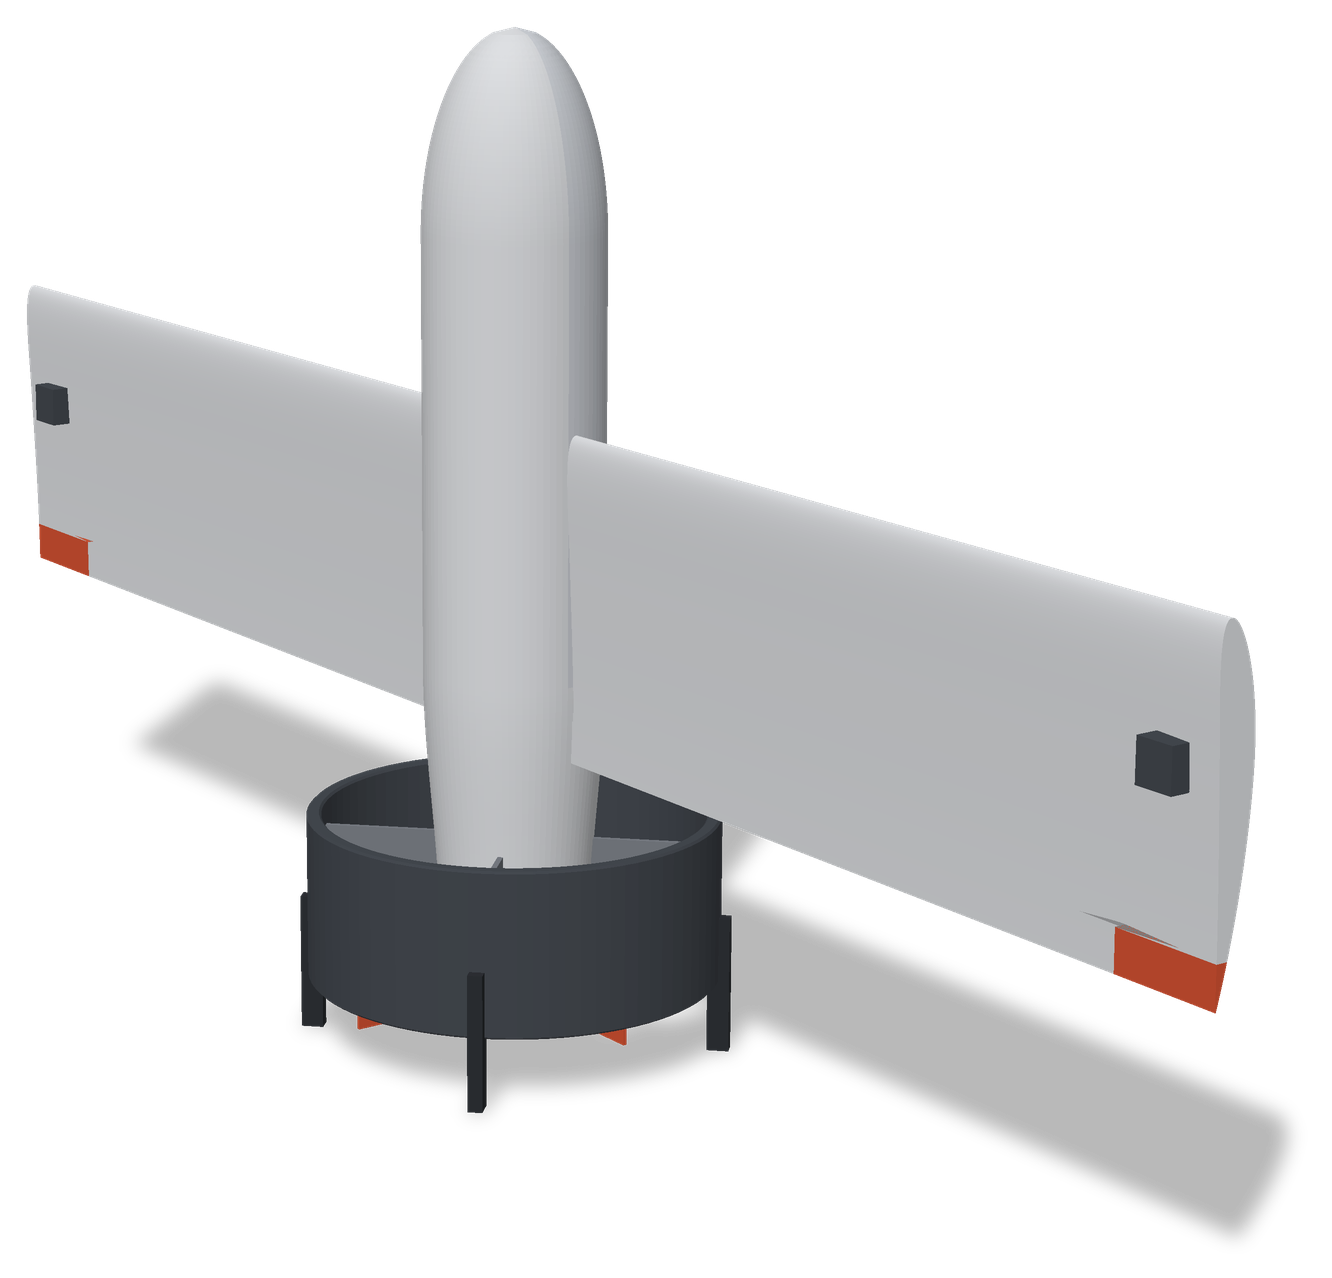
\includegraphics[width=\linewidth]{vbat_render}
  \caption{Rendered vehicle, tail-down on its landing legs.}
\end{subfigure}\hfill
\begin{subfigure}[t]{0.48\textwidth}
  \centering
  
\includegraphics[width=\linewidth]{fuselage_layout}
  \caption{Fuselage packaging and bay stack from the layout stage.}
\end{subfigure}
\caption{Pipeline-generated design artifacts: every figure is
regenerated from configuration by the deterministic pipeline; none is
hand-drawn.}
\label{fig:vehicle}
\end{figure}

The commercial-component freeze (pipeline stage 12) selected, against
requirements \emph{derived} from the converged design point, a
Pixhawk-class PX4 flight controller, a telemetry-capable 80\,A-class
ESC, the pinned 3-blade $8\times6$ propeller, sub-10\,g-class
control-surface servos, and a 21700 Li-ion 6S pack that undercuts the
sized LiPo pack by $\sim$203\,g --- flipping the as-selected all-up
mass 182\,g \emph{below} the conceptual closure. The as-selected
re-solve (stages 13--15) then re-solved the affected subsystems with
real hardware masses and envelopes and confirmed physical fit in the
unchanged $\varnothing$107\,mm hull.

Crucially, the pipeline also reports what does \emph{not} close.
Standing findings pinned at the final snapshot include: a marginal ESC
cold plate (its $\sim$37\,W hover load needs a plate heavier than the
ESC mass allocation, with only a few $^{\circ}$C margin); a battery
pack that, at the 40\,$^{\circ}$C design ambient and nominal
90\,m$\Omega$ resistance, ends the mission $\sim$5\,$^{\circ}$C over
its 60\,$^{\circ}$C limit (making measured pack resistance a
procurement acceptance criterion); and avionics-bay and motor mass
allocations exceeded by $\sim$25\,g and $\sim$79\,g respectively.
These are carried openly as accepted risks with named retirement
paths, not tuned away --- the behavior the standing-findings
discipline of Section~\ref{sec:verification} was designed to produce.

\subsection{Design-point evolution}
\label{sec:evolution}

Table~\ref{tab:evolution} traces the design point across the tagged
snapshots. The trajectory is deliberately non-monotonic: the design
got \emph{heavier} whenever a model was made more honest (the
3D-printability penalty at v0.2.0; the battery internal-resistance
accounting at v0.5.1, $+215$\,g) and lighter whenever architecture or
procurement evidence justified it (the externally reviewed
semi-monocoque re-baseline at v0.4.0; the larger, lower-disk-loading
propeller the component freeze forced at v0.4.1). Each row is a
complete, internally consistent, released design snapshot with its
regression pins, CFD references, CAD exports, and changelog updated in
the same change --- there is no intermediate state in the history in
which the artifacts disagree.

\begin{table}[htbp]
\centering
\caption{Design-point evolution across tagged snapshots. Every row is
a fully re-converged, regression-pinned release.}
\label{tab:evolution}
\small
\begin{tabularx}{\textwidth}{@{}llllX@{}}
\toprule
\textbf{Tag} & \textbf{Date} & \textbf{MTOW} & \textbf{Hover} &
\textbf{Driver of the change} \\
\midrule
v0.1.0 & Jul 09 & 2.50\,kg & $\sim$770\,W &
Initial closure: NACA 2412 wing, 195\,mm COTS fan assumption \\
v0.2.0 & Jul 10 & 3.06\,kg & $\sim$1030\,W &
Honest 3D-printed-structure penalty enters the closure; vibration
isolation and modularity split lines added \\
v0.3.0 & Jul 10 & 3.06\,kg & --- &
Thermal paths sized as structure; marginal ESC cold plate first
reported as a standing finding \\
v0.4.0 & Jul 11 & 2.376\,kg & 710\,W &
Semi-monocoque clamshell fuselage from independent expert review;
structural budget re-baselined to an explicit member model \\
v0.4.1 & Jul 15 & 2.302\,kg & 652\,W &
Component freeze reveals the 195\,mm fan class is unbuyable at this
scale; propulsion decision amended by ADR to a 203\,mm 3-blade
propeller in the airframe duct \\
v0.4.5 & Jul 17 & 2.303\,kg & --- &
Li-ion 21700 pack wins the battery freeze; battery mission-transient
thermal check added from external review \\
v0.5.0 & Jul 17 & 2.303\,kg & --- &
Stall-speed inconsistency found by expert review (placeholder
$C_{L,\max}$ survived in one report); wing re-sized to the real
airfoil limit \\
v0.5.1 & Jul 19 & 2.518\,kg & 743\,W &
NACA 4412 re-selection exploits the now-honest stall constraint;
pack $I^2R$ losses folded into closure ($+215$\,g accepted) \\
v0.5.2 & Jul 21 & 2.518\,kg & 743\,W &
Versioned aerodynamic hand-off contract iterated with the external
solver consumer (six schema releases) \\
\bottomrule
\end{tabularx}
\end{table}

\subsection{Process evidence: quantifying the AI's role}
\label{sec:process-results}

Because every AI-implemented commit carries a machine-readable
co-authorship trailer, the division of labor is recoverable directly
from the git history, providing unusually direct process evidence.

\paragraph{Two phases, one repository.} The project history contains a
natural comparison. In a first, entirely manual phase (4~February --
27~March), 28 commits over seven calendar weeks carried the study
through mission sizing, initial take-off-weight iteration, airfoil
selection, and control-vane design --- roughly the first three of the
eventual sixteen pipeline stages, with physics gradually migrating out
of notebooks. In the AI-assisted phase (4--24~July), 109 commits over
three calendar weeks of part-time work delivered the remaining
thirteen pipeline stages plus the full governance and verification
infrastructure: parametric CAD, CFD cases, vibration, thermal, mass
properties, wiring, component freeze, the as-selected re-solve,
sixteen executed notebooks in CI, 147 pinned regression tests, and
thirteen tagged design releases (v0.1.0 through v0.5.2 in twelve
days). While the two phases are not perfectly controlled (the second
benefited from the first's groundwork), the contrast in scope per
calendar week is roughly an order of magnitude and is consistent with
the acceleration claims in the surrogate-model literature, achieved
here at the workflow level rather than inside a single discipline.

\paragraph{Contribution split.} Of the 109 AI-phase commits, 70
(64\%) carry AI co-authorship trailers; the remainder are human-only
commits (merges, reviews, manual fixes, procurement research). All 23
engineering pull requests of the AI phase were human-reviewed before
merge. The final repository comprises $\sim$11{,}200 lines of
deterministic physics library code, $\sim$1{,}800 lines of tests, 18
commented configuration files, 16 orchestration notebooks, and 18
architecture decision records --- the ADRs and changelog entries
drafted by the agent as part of the changes they document.

\paragraph{Error-catching channels.} The history also documents
\emph{which} safety net caught each class of error, summarized in
Table~\ref{tab:errors}. The pattern is consistent with the layered
design of Section~\ref{sec:method}: automated pins caught silent
drift, schema-governed hand-offs caught cross-tool integration faults,
and independent human expertise caught conceptual errors invisible to
any automated check --- confirming that expert review is a
load-bearing element of the methodology, not a formality.

\begin{table}[htbp]
\centering
\caption{Representative faults during the case study and the
methodology layer that caught each.}
\label{tab:errors}
\small
\begin{tabularx}{\textwidth}{@{}XX@{}}
\toprule
\textbf{Fault} & \textbf{Caught by} \\
\midrule
Propulsion/vane CFD cases silently meshing an obsolete design point &
Cross-consumer consistency discipline; cases re-sourced from hand-offs
with a design-point stamp that refuses stale reuse \\
\addlinespace
Stall requirement silently unmet (placeholder $C_{L,\max}$ vs.\
selected airfoil) & Independent expert review (v0.5.0) \\
\addlinespace
Unrealistically optimistic battery efficiency (implied
$\sim$23\,m$\Omega$ pack) & Expert review prompting the transient
model; closure re-derived from pack physics (v0.4.5--v0.5.1) \\
\addlinespace
Wing control points inside the fuselage in the external solver &
Versioned hand-off schema iteration with the consumer (placement
anchor made mandatory from schema 1.5.0) \\
\addlinespace
Unbuyable propulsion assumption (195\,mm fan class) & Deterministic
component-freeze stage; assumption amended by ADR (v0.4.1) \\
\addlinespace
Refactoring risk while moving physics out of notebooks &
Byte-identical hand-off verification (ADR-0013, ADR-0018) \\
\bottomrule
\end{tabularx}
\end{table}

\subsection{Discussion}
\label{sec:discussion}

\paragraph{Answering the research question.} The case study supports
an affirmative, but conditional, answer to the RQ. The AI accelerated
the program by roughly an order of magnitude in delivered scope per
calendar week --- but the acceleration was \emph{not} obtained by
letting the model produce engineering answers. Every number in
Table~\ref{tab:designpoint} traces to deterministic, configured,
regression-tested physics; the AI's leverage came from (i)
implementing multidisciplinary changes completely, so that a design
move lands with its pins, consumers, decision record, and changelog in
one reviewable diff; (ii) eliminating the bookkeeping latency that
normally separates a design decision from a fully consistent design
state; and (iii) making honest-model refinements cheap enough that
unfavorable results (a $+215$\,g mass growth, a marginal cold plate)
were adopted rather than resisted.

\paragraph{Division of labor.} The observed equilibrium assigns the
AI what LLM agents are reliably good at --- exhaustive propagation,
code implementation, documentation, consistency --- and reserves for
humans what they were uniquely necessary for in this program:
requirement setting, acceptance of every decision, procurement
judgment, and conceptual review. It is notable that both of the case
study's most consequential errors (the stall inconsistency and the
optimistic battery efficiency) were latent \emph{before} the AI phase
and were surfaced during it, one by human expert review and one by an
expert-prompted model refinement the AI then implemented. Neither the
AI alone nor the automation alone would have sufficed; the methodology
is precisely the structure that lets each catch what the other misses.

\paragraph{Generality.} Nothing in
Sections~\ref{sec:pipeline}--\ref{sec:iteration} is specific to
tail-sitters: the constitution, one-way pipeline, pins, ADR
discipline, and interaction protocol transfer directly to any
configuration-driven engineering program with computable analysis
stages. The tail-sitter case exercised the framework hard ---
hover/cruise coupling, dual control effectors, thermal and vibration
constraints, and a procurement reality check all interact --- which is
exactly why it was chosen as the validation vehicle.

\paragraph{Limitations.} The study is a single case with a team
already expert in the domain and the tooling; the phase comparison is
suggestive, not controlled. All analyses are conceptual-level
(momentum theory, lifting-line-class aerodynamics, first-order thermal
and structural models); transition dynamics are energetically budgeted
but not simulated, and no hardware has flown --- the PX4-based flight
validation and the external VLM/BEMT and CFD loops are the designed
next steps, wired into the same hand-off contracts. Finally, the
methodology's guardrails bound, but cannot eliminate, LLM
fallibility: the protection is structural (nothing merges without
passing pins, CI, and human review), and the residual risk
concentrates exactly where automated checks are weakest ---
conceptual assumptions --- which is why independent expert review
remains mandatory in the loop.

\section{Conclusions}
\label{sec:conclusions}

This paper introduced a structured methodology for AI-assisted
conceptual aircraft design in which a large-language-model agent works
as an engineering collaborator inside a governed, version-controlled
design repository. The methodology rests on a strict separation of
roles --- deterministic, configured, regression-tested physics code as
the sole source of engineering numbers; the AI as the implementer and
propagator of design changes; humans as the source of requirements,
directives, review, and acceptance --- enforced by four transferable
mechanisms: a machine-readable project constitution, a one-way
analysis pipeline with typed hand-offs, pinned design-point regression
tests with full-pipeline continuous integration, and architecture
decision records with git-level provenance of AI contribution.

Applied to the conceptual design of a small electric tail-sitter VTOL
UAV, the methodology carried the program from mission requirements to
a converged, commercially frozen 2.52\,kg design point --- sixteen
analysis stages spanning sizing, aerodynamics, control authority,
vibration, thermal, CAD, component selection, and higher-fidelity
hand-off --- in three calendar weeks of part-time work, with thirteen
fully consistent tagged design snapshots and eighteen recorded
architecture decisions. Process evidence extracted from the git
history shows 64\% of design-phase commits co-authored by the AI, all
merged through human review, and documents which safety layer caught
each class of fault: automated pins caught silent drift, versioned
hand-off schemas caught cross-tool integration errors, and independent
expert review caught the conceptual errors no automated check could
see.

The answer to the research question is therefore affirmative but
conditional: AI can accelerate conceptual aircraft design by roughly
an order of magnitude in delivered scope per unit time \emph{when} it
is deployed at the workflow level under structural guardrails, rather
than as a source of engineering answers. The acceleration was used not
to cut corners but to make honesty cheap --- model refinements that
grew the design mass were adopted within days, and unfavorable margins
are carried openly as standing findings with named retirement paths.

Future work proceeds along the hand-offs the methodology already
exposes: closing the external vortex-lattice/blade-element and CFD
loops on the frozen geometry, PX4-based flight validation of the
hover/transition control architecture, folding measured component
properties (notably pack internal resistance) back into the closure
after procurement, and applying the framework to a second, dissimilar
airframe to test aircraft-independence. On the methodological side,
controlled multi-team studies are needed to separate the contributions
of the AI agent, the governance structure, and team expertise to the
observed acceleration.


\section*{Acknowledgements}
An LLM-based coding agent (Claude Code; Anthropic) was used throughout
this work as the AI engineering collaborator whose use is the subject
of this paper: it implemented and refactored the physics modules,
executed the design pipeline, drafted architecture decision records,
and assisted in drafting this manuscript under the direction and review
of the authors. Literature retrieval was assisted by the Consensus
academic search engine. All engineering results were produced by the
deterministic, version-controlled analysis code described in
Section~\ref{sec:method}, and all content was reviewed and verified by
the human authors, who take full responsibility for it.

\bibliographystyle{plainnat}
\bibliography{references}

\end{document}
